\documentclass[aspectratio=169,12pt]{beamer}
\usetheme{Boadilla}
\setbeamertemplate{blocks}[default]
\setbeamertemplate{itemize items}[default]
\setbeamertemplate{enumerate items}[default]
\setbeamertemplate{bibliography item}{\insertbiblabel}
\setbeamertemplate{section in toc}{\inserttocsectionnumber.~\inserttocsection}
\setbeamertemplate{navigation symbols}{}
\usecolortheme{crane}
\usepackage[french]{babel}
\usepackage[utf8]{inputenc}
\usepackage[T1]{fontenc}
\usepackage{listings} 
\usepackage{color}
\usepackage{xcolor}
\newcommand\go{``}
\newcommand\gf{''}
\newcommand{\guille}[1]{\go#1\gf}
\usepackage[sfdefault,light]{FiraSans}
\usepackage[style=numeric,
bibstyle=numeric,
backend=bibtex]{biblatex}
\addbibresource{bibliography.bib}
\graphicspath{{images/}}
% Define the "Bootlin blue" color
\definecolor{commentcolor}{RGB}{170,170,170}
\definecolor{identifiercolor}{RGB}{170,55,49}
\definecolor{keywordcolor}{RGB}{75,105,198}
\definecolor{stringscolor}{RGB}{156,93,39}
\definecolor{fedarkblue}{rgb}{0.25,0.25,0.75}
\setbeamercolor{darkblue}{fg=fedarkblue}
%\hypersetup{colorlinks,linkcolor=,urlcolor=fedarkblue}

% Custom Bootlin commands
\newcommand{\code}[1]{{\usebeamercolor[fg]{darkblue} \path{#1}}}

\lstdefinestyle{customc}{
	breaklines=true,
	tabsize=2,
	frame=lines,
	%xleftmargin=\parindent,
	language=C,
	numbers=left,
	numbersep=.15cm,
	numberstyle=\footnotesize\ttfamily,
	numberblanklines=true,
	showstringspaces=false,
	basicstyle=\footnotesize\ttfamily,
	%backgroundcolor = \color{lightgray!10},
	keywordstyle=\bfseries\color{keywordcolor},
	commentstyle=\itshape\color{commentcolor},
	identifierstyle=\color{identifiercolor},
	stringstyle=\color{stringscolor},
}

\title{Main title}
\subtitle{Subtitle if needed}
\author{Pascal Cotret, ENSTA Bretagne} 
\date{\today}

\begin{document}
	\frame[plain]{\titlepage} 
	
	\begin{frame}{title}
		\begin{itemize}
			\item \code{code}\cite{Feynman1941}
			\item \code{code2}\footfullcite{Arias2020}
			\item \code{code3}
		\end{itemize}
		\begin{enumerate}
			\item un
			\item deux
			\item trois
		\end{enumerate}
	\end{frame}
	
	\begin{frame}{title}
		\begin{block}{block}
			content
		\end{block}
		\begin{exampleblock}{exampleblock}
			content
		\end{exampleblock}
		\begin{alertblock}{alertblock}
			content
		\end{alertblock}
	\end{frame}
	
	\begin{frame}[fragile]{Example of embedded code}
		\begin{lstlisting}[style=customc]
int fib(int n){
	if (n < 2)
		return n;
	else
		return fib(n-1) + fib(n-2);
	}
	// Print Fibonacci value
	printf("%d\n", fib(10));
\end{lstlisting}
	\end{frame}
	
	\begin{frame}{}
		\begin{figure}[htbp]
			\centering
			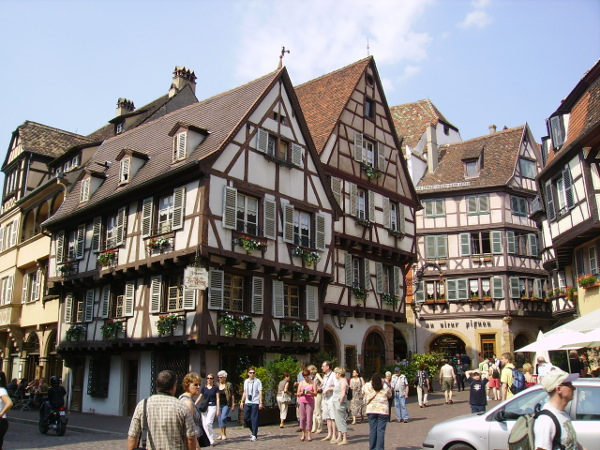
\includegraphics[width=.5\textwidth]{alsace}
			\caption{Maison colmarienne}
		\end{figure}
	\end{frame}
	
	\begin{frame}{Références}
		\printbibliography
	\end{frame}
\end{document}